%!TEX TS-program = xelatex
\documentclass[]{friggeri-cv}
\usepackage[a4paper, total={6in, 8in}, margin=0.5in]{geometry}
\usepackage{afterpage}
\usepackage{hyperref}
\usepackage{color}
\usepackage{xcolor}
\usepackage{smartdiagram}
\usepackage{fontspec}
% if you want to add fontawesome package
% you need to compile the tex file with LuaLaTeX
% References:
%   http://texdoc.net/texmf-dist/doc/latex/fontawesome/fontawesome.pdf
%   https://www.ctan.org/tex-archive/fonts/fontawesome?lang=en
%\usepackage{fontawesome}
\usepackage{metalogo}
\usepackage{dtklogos}
\usepackage[utf8]{inputenc}
\usepackage{tikz}
\usetikzlibrary{mindmap,shadows}
\hypersetup{
    pdftitle={},
    pdfauthor={},
    pdfsubject={},
    pdfkeywords={},
    colorlinks=false,           % no lik border color
    allbordercolors=white       % white border color for all
}


\smartdiagramset{
    bubble center node font = \footnotesize,
    bubble node font = \footnotesize,
    % specifies the minimum size of the bubble center node
    bubble center node size = 0.4cm,
    %  specifies the minimum size of the bubbles
    bubble node size = 0.1cm,
    % specifies which is the distance among the bubble center node and the other bubbles
    distance center/other bubbles = 0.5cm,
    % sets the distance from the text to the border of the bubble center node
    distance text center bubble = 0.1cm,
    % set center bubble color
    bubble center node color = lblue,
    % define the list of colors usable in the diagram
    set color list = {lightgray, materialcyan, orange, green, materialorange, materialteal, materialamber, materialindigo, materialgreen, materiallime},
    % sets the opacity at which the bubbles are shown
    bubble fill opacity = 0.4,
    % sets the opacity at which the bubble text is shown
    bubble text opacity = 1,
}

\addbibresource{bibliography.bib}
\RequirePackage{xcolor}
\definecolor{pblue}{HTML}{006699}
\definecolor{lblue}{HTML}{0099CC}

\begin{document}
\header{\hspace{15mm}}{ Jimson Gelbolingo Ngeo\\}
       {Information Science Engineer}
      
% Fake text to add separator  
\vspace{-5mm}
\fcolorbox{white}{gray}{\parbox{\dimexpr\textwidth-2\fboxsep-2\fboxrule}{%
.....
}}

% In the aside, each new line forces a line break
\begin{aside}
  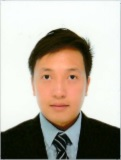
\includegraphics[scale=0.8]{img/JimsonNgeo_3x4photo.jpg}
  \section{Address}
    Chiba-ken Chiba-shi Mihama-ku
    Masago 5-16-4-401
    ~
  \section{Tel}
    +81 80 4240 0512
    ~
  \section{Mail}
    \href{mailto:jimsonngeo@gmail.com}{\textbf{jimsonngeo@}\\gmail.com}
    ~
  \section{Web}
    \href{https://www.linkedin.com/in/jngeo/}{https://linkedin.com/\\in/jngeo/}
%    \href{https://bitbucket.org/mygit}{bitbucket.org/mygit} https://www.linkedin.com/in/jngeo/
    ~
  % use  \hspace{} or \vspace{} to change bubble size, if needed
  \section{Skills}
    \smartdiagram[bubble diagram]{
        \textbf{Information}\\\textbf{Science},
        \textbf{Machine}\\{Learning},
        \textbf{Sensor}\\{Fusion},
        \textbf{Signal}\\\textbf{Processing},
        \textbf{Statistical}\\\textbf{Analysis},
        \textbf{Optimi-}\\\textbf{zation}
    }
    ~
    % Programming skill bar
    \section{Programming}
        \begin{tikzpicture}
            \draw[fill=maingray,maingray] (0,0) rectangle (3.5,0+0.4);
			\draw[fill=white,mainblue](0,0) rectangle (3.5,0+0.4);
			\node[above right] at (0,0+0.35) {Matlab $\textbullet$ Python};
        \end{tikzpicture}
        \begin{tikzpicture}
            \draw[fill=maingray,maingray] (0,1) rectangle (3.5,1+0.4);
			\draw[fill=white,mainblue](0,1) rectangle (3,1+0.4);
			\node[above right] at (0,1+0.35) {C$\textbackslash$C++ $\textbullet$ QT};
        \end{tikzpicture}
        \begin{tikzpicture}
            \draw[fill=maingray,maingray] (0,2) rectangle (3.5,2+0.4);
			\draw[fill=white,mainblue](0,2) rectangle (2.5,2+0.4);
			\node[above right] at (0,2+0.35) {HTML $\textbullet$ \large \LaTeX};
        \end{tikzpicture}
    ~
\end{aside}

~
\section{Experience}
\begin{entrylist}
  \entry
    %{Apr 2016 - present\\}
    {2016 - present\\}
    {Operations Engineer}
    {\href{{https://global.weathernews.com/your-industry/shipping/}}{{Weathernews, Inc., Japan}}}
    {Provides 24/7 weather communication setup to marine vessels around the world to ensure safe and efficient operations through weather data-driven technological solutions.
    \\}
  \entry
    %{Aug 2017 - present\\}
    {2017 - 2018}
    {Technology Consultant}
    {\href{{ https://ximity.net/}}{{Ximity Inc., Philippines}}}
    {Supports product development of next generation Internet-of-Things (IoT) applications for the Philippine market, mainly focusing on Low Power Wide Area Network (LORAWAN) applications.
    \\}
  \entry
    %{Oct 2014 - Mar 2016 \\}
    {2014 - 2016}
    {Special Researcher}
    {\href{{http://www.brain.kyutech.ac.jp/~tom/member/}}{{Kyushu Institute of Technology, Kitakyushu Japan}}}
    {Under the Human and Social Intelligence Systems Lab, trained PhD and Master students in machine learning applications and handling of specialized equipment. High experience in working with Gaussian Processes, Neural Networks and time-series and spatial-temporal data.
    \\}
  \entry
    %{Apr 2008 - Mar 2010 \\}
    {2008 - 2010}
    {Assistant Instructor}
    {\href{{https://www.ateneo.edu/ls/sose}}{{Ateneo de Manila University, Philippines}}}
    {Under the Department of Electronics, Computer and Communications Engineering, taught undergraduate courses in mathematics, telecommunications and electronics. Led research groups in developing biomedical applications.
    }
\end{entrylist}

\\\\

\section{Education}
\begin{entrylist}
\entry
    {2013 - 2016}      
    {PhD in Information Science}
    {\href{{http://www.naist.jp/en/}}{{Nara Institute of Science and Technology, Japan}}}
    {Conducted research and published several articles and journals in Biomedical and Neuro-Engineering, specifically on Modeling dynamic and high degree-of-freedom finger kinematics from surface electromyographic (EMG) signals. Specialization is on machine learning, signal processing and sensors.
    \\}
\entry
    {2011 - 2013}      
    {Master in Information Science}
    {\href{{https://sites.google.com/view/milab/home}}{{Nara Institute of Science and Technology, Japan}}}
    {Conducted research and published academic papers in Rehabilitation and Neuro-engineering, specifically on continuous estimation of finger joint angles using muscle activation inputs from EMG signals.
    \\}
\entry
    {2010}
    {Japanese Language Training  Course}
    {Osaka University, Japan}
    {Participated in an intensive Japanese language course for beginners in preparation for graduate school.
    \\}
\entry
    {2003 - 2008}
    {BS in Electronics and Communications Engineering\\}
    {\href{{https://www.ateneo.edu/ls/sose}}{{Ateneo de Manila University, Philippines}}}
    {}
    {}
    %{For the Bachelor's thesis, worked on projects involving electronics, biomedical application and signal processing
    %\\}
\end{entrylist}


\newpage

\begin{aside}
  ~
%  \section{Places Lived}
%    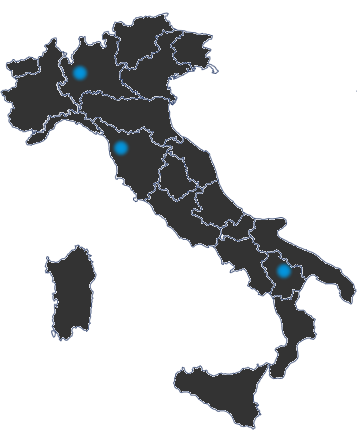
\includegraphics[scale=0.25]{img/italia.png}*/
%    ~
  \vspace{10mm}
  \section{Languages}
    \textbf{English}
\includegraphics[scale=0.40]{img/5stars.png}
    \textbf{Filipino}
\includegraphics[scale=0.40]{img/5stars.png}
    \textbf{Chinese}
\includegraphics[scale=0.40]{img/3stars.png}
    \textbf{Japanese}
\includegraphics[scale=0.40]{img/2stars.png}
    ~
\end{aside}


%\begin{entrylist}
%  \entry
%    {2003 - 2008}
%    {Bachelor's Degree in Electronics and Communications Engineering\\}
%    {Ateneo de Manila University, Philippines}
%    {For the Bachelor's thesis, worked on projects involving electronics, biomedical application and signal processing.}
%\end{entrylist}


\section{Publications}
J. Ngeo, T. Tamei and T. Shibata\\
\textbf{Continuous and simultaneous estimation of finger kinematics
using inputs from an EMG-to-muscle activation model}\\
\small{\emph{In: Journal of NeuroEngineering and Rehabilitation, 11:122, 2014}}
\\
\\
J. Ngeo, T. Tamei, K. Ikeda and T. Shibata\\
\textbf{Modeling dynamic high-DOF finger postures
from surface EMG using nonlinear synergies in latent space representation}\\
\small{\emph{In: Proceedings of the 37th Annual International Conference of the IEEE Engineering in Medicine and Biology Society (EMBC), Milano, Italy, Aug 25–29, 2015}}
\\
\\
 N. Koganti, J. Ngeo, T. Tamei, K. Ikeda and T. Shibata\\
\textbf{Cloth dynamics modeling in latent spaces and its application to robotic clothing assistance}\\
\small{\emph{In: IEEE/RSJ International Conference on Intelligent Robots and Systems (IROS 15), Hamburg, Germany, 2015}}
\\
\\
J. Ngeo, T. Tamei and T. Shibata\\
\textbf{Estimation of continuous multi-DOF finger joint kinematics from surface EMG using a multi-output GP}\\
\small{\emph{In: Proceedings of the 36th Annual International Conference of the IEEE Engineering in Medicine and Biology Society (EMBC), Chicago, USA, Aug 26–30, 2014}}
\\
\\
J. Ngeo, T. Tamei, T. Shibata, M.F. Orlando, L. Behera, A. Saxena and A. Dutta\
\textbf{ Control of an Optimal Finger Exoskeleton based on Continuous Joint Angle Estimation from EMG signals}\\
\small{\emph{In: Proceedings of the 35th Annual International Conference of the IEEE Engineering in Medicine and Biology Society (EMBC), Osaka, Japan, Jul 3–7, 2013}}
\\
\\
J. Ngeo, T. Tamei and T. Shibata\\
\textbf{Continuous Estimation of Finger Joint Angles Using Muscle Activation Inputs from Surface EMG Signals}\\
\small{\emph{In: Proceedings of the 34th Annual International Conference of the IEEE Engineering in Medicine and Biology Society (EMBC), San Diego, USA, Aug 28–Sep 1, 2012}}

%\\
%R. Reyes, J. Monje, M. Santos, L.A. Mateo, R. Espiritu, J. Isiderio, C.M. Lacson, and R. Ocfemia\\
%\textbf{Throughput and Power Consumption Comparisons of Zigbee-based and ISM-based Implementations of WSAN}\\
%\emph{In NAUN International Journal of Communications, 4(3):96–104, 2009}
%\\
\section{Honors \& Awards}
\begin{entrylist}
  \entry
    {2015}
    {IROS 2015} 
    {Best Application Paper Award}
    {\emph{Title:Cloth dynamics modeling in latent spaces and its application to robotic clothing assistance. In: IEEE/RSJ International Conference on Intelligent Robots and Systems}}
  \entry
    {2015}
    {IEEE-EMBS Summer School 2015} 
    {Best Poster Presentation Award}
    {\emph{Paper Title:Continuous and simultaneous estimation of finger kinematics using inputs from an EMG-to-muscle activation model}}
  \entry
    {2010 - 2016}
    {Japanese Government Scholarship}
    {Research, M.S. and PhD Scholarships}
    {\emph{Granted by the Monbukagakusho Scholarship Program}}
    
  \entry
    {2012}
%    \href{https://cicp.naist.jp/ja/}
    {Creative and International Competitiveness Project 2012}
    {2nd Prize}
    {\emph{Entry: An Anonymous and Intelligent Message Broadcasting Service for smartphone and handheld game console users, details \href{https://cicp.naist.jp/ja/}{here}}}
  \entry
    {2010}
%    \href{https://www.fishermanfoundation.com/hapinoy.html}
    {Hapinoy Fisherman Breakthrough Innovation}
    {3rd Prize}
    {\emph{Entry: Hapinoy Tingi Tawag Abroad (VOIP call station) for Philippine communities with insufficient IT infrastructure, details \href{https://www.fishermanfoundation.com/hapinoy.html}{here}}}
   \entry
    {2008}
    {4th Smart Wireless Engineering Education Program (SWEEP) Award}
    {3rd Prize}
    {\emph{Project on Smart Guards, a disease and epidemic tracking and alert system}}
\end{entrylist}

%\section{Certifications}
%\begin{entrylist}
%  \entry
%    {02/2013}
%   {Intro to Computer Science}
%    {Udacity. E-learning}
%    {\emph{Building a Python Search Engine}}
%\end{entrylist}

%\section{Other Info}
%For the Italian job market:\\
%\emph{Si autorizza il trattamento delle informazioni contenute nel curriculum in conformità alle disposizioni previste dal d.lgs. 196/2003. Si dichiara altresì di essere consapevole che, in caso di dichiarazioni non veritiere, si è passibili di sanzioni penali ai sensi del DPR 445/00 oltre alla revoca dei benefici eventualmente percepiti.}
%\\
%\begin{flushleft}
%\emph{March 2018}
%\end{flushleft}
%\begin{flushright}
%\emph{Lorlynn Asuncion Mateo}
%\end{flushright}

\end{document}
